\documentclass[conference]{IEEEtran}
\IEEEoverridecommandlockouts
% The preceding line is only needed to identify funding in the first footnote. If that is unneeded, please comment it out.
\usepackage{cite}
\usepackage[utf8]{inputenc}
\usepackage{amsmath,amssymb,amsfonts}
\usepackage{algorithmic}
\usepackage{graphicx}
\usepackage{textcomp}
\usepackage{lipsum}
\usepackage{xcolor}
\usepackage{caption}
\usepackage{array}

\captionsetup[table]{name=Tabela}
\def\BibTeX{{\rm B\kern-.05em{\sc i\kern-.025em b}\kern-.08em
		T\kern-.1667em\lower.7ex\hbox{E}\kern-.125emX}}
\begin{document}
	
\title{Register Transfer Level and High Level Synthesis Implementation of Correlation measure focused on small number of features\\
	}

\author{\IEEEauthorblockN{1\textsuperscript{st} Pedro Lucas Falcão Lima}
	\IEEEauthorblockA{\textit{Departamento de Teleinformática (DETI)} \\
		\textit{Universidade Federal do Ceará (UFC)}\\
		Fortaleza, Brasil \\
		pedrolfalc@gmail.com}
	\and
	\IEEEauthorblockN{2\textsuperscript{nd} Given Name Surname}
	\IEEEauthorblockA{\textit{dept. name of organization (of Aff.)} \\
		\textit{name of organization (of Aff.)}\\
		City, Country \\
		email address}
	\and
	\IEEEauthorblockN{3\textsuperscript{th} Given Name Surname}
	\IEEEauthorblockA{\textit{dept. name of organization (of Aff.)} \\
		\textit{name of organization (of Aff.)}\\
		City, Country \\
		email address}
	
}

\maketitle
	\begin{abstract}
					
	Sistemas de detecção de intrusão são cada vez mais necessários para garantir a segurança
	de serviços na internet, uma vez que as ameaças na rede vem desenvolvendo-se cada
	vez mais. Ataques do tipo DDoS são muito comuns atualmente, uma vez que já existem
	recursos suficientes para realizar esse tipo de ataque em tempo real. Apesar de existirem
	soluções em softwares para detectar ataques DDoS, muitas são ineficientes. Nesse trabalho
	foi implementado um soft ip core para FPGAs que realiza a detecção de ataque DDoS
	em tempo real, em um tempo de menos de 1 $\mu$s. Além disso, o módulo implementado alia
	baixa utilização de recursos, pois faz uso de aritmética de ponto fixo, com uma elevada
	precisão quando comparado a implementação em software com ponto flutuante. O módulo
	foi implementado de duas formas em nível RTL e utilizando uma ferramenta de implementação e otimização utilizando IP's. Ambas os métodos foram sintetizado em uma FPGA Artix da Série 7 da Xilinx.
		
	\end{abstract}
	
	
	\renewcommand{\IEEEkeywordsname}{Palavras-chave}
	\begin{IEEEkeywords}
		Módulo,FPGA, Segurança, Tempo Real, Correlação, Hardware.
	\end{IEEEkeywords}
	
	\section{Introdução}
	
	
Devido a complexidade das aplicações modernas, sistemas de tempo real são cada vez mais necessários no contexto atual. Tais sistemas estão incluídos nas mais variadas áreas de conhecimento: Aviação, medicina, astronomia e etc. Sabendo que esses sistemas requerem velocidade e desempenho, além alto grau de processamento é importante novos métodos e tecnologias para otimização das aplicações de tempo real.\\
Os métodos de otimização de sistemas de tempo real são baseados na metodologia em que esses sistemas são implementados(algoritmos,métricas e fluxo). Além disso, existem estratégias que buscam realizar otimização em sistemas sem afetar a estrutura do mesmo. Vale ressaltar, que a otimização ideal ocorre para todos os requisitos da aplicação, porém em sistemas reais devem existir requisitos mais prioritários para que haja um maior ganho específico nos fins que a aplicação deseja realizar.\\
Para realizar tarefas de alto grau de processamento é necessário algumas estratégias podem ser utilizadas como utilização de funções matemáticas consolidadas, métodos estatísticos tradicionais e novos algoritmos. Porém para esse processamento ser em tempo real ele deve ser dinâmico e veloz por isso em pouco tempo ele deve processar um conjunto de dados em um sistema. Por isso um método simples de otimização seria a redução variáveis de entrada para a realização dessa tarefa, assim alocando o máximo de tempo possível para o processamento dessas entradas no sistema.\\
As tecnologias baseadas em software são ineficientes para aplicações de tempo real, uma vez que eles exigem grande quantidade de ciclos de CPU de propósitos gerais. Logo, é necessário que soluções em hardware estejam presentes nas soluções de sistema de tempo real. Podendo assim, ser gerados sistemas híbridos (hardware e software) que possuem alto desempenho e precisão. \\
Os tipos de Hardware que possuem características para acomodar grandes lógicas e possuem alto poder de processamento são as FPGAs e ASICs, porém as FPGAs oferecem adaptabilidade dinâmica, que é importante para aplicações que requerem mudanças frequentes em suas configurações.

	
	\section{Detalhamento Técnico}
	A NoC Phoenix \cite{b7} é uma arquitetura de PEs intrachip, podendo atuar sobre uma plataforma de processadores (em inglês, MultiProcessor SoC - MPSoC), que utiliza uma topologia com malha 2D como infraestrutura de comunicação, sua divisão consiste em uma parte hardware chamada HwPhoenix (roteadores) e uma parte software chamada OsPhoenix (sistema operacional de cada PE)  (Figura\ref{ArquiteturaBasica}). Basicamente a Phoenix possui uma topologia de  dimensões m × n com roteadores que são conectados entre si por meio de links bidirecionais, sendo que cada roteador possui cinco portas: Norte, Sul, Leste, Oeste e Local(interface de rede).\\
	
	\begin{figure}[htbp]
		\centerline{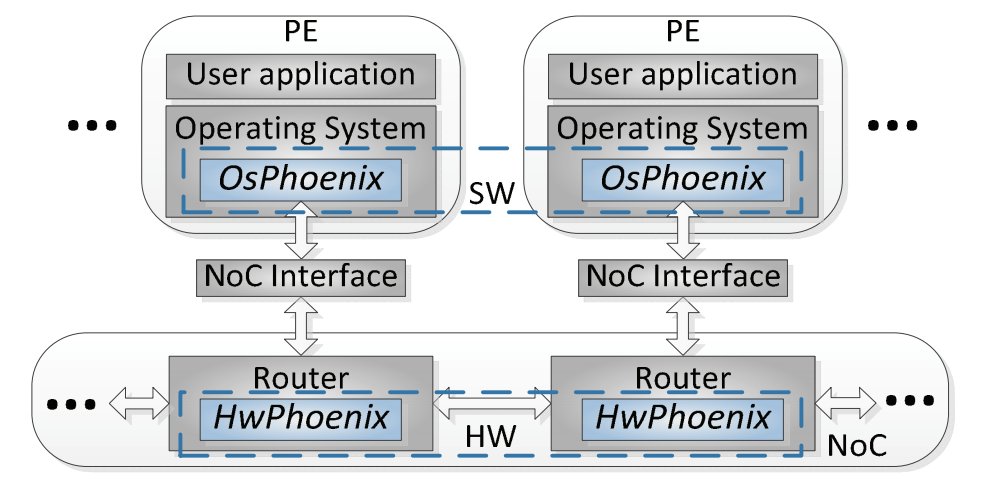
\includegraphics[scale=0.365]{fig1.jpg}}
		\caption{Arquitetura básica Phoenix (contendo HwPhoenix e OSPhoenix)}
		\label{ArquiteturaBasica}
	\end{figure}
	
	Para realizar uma significativa melhora na eficiência da NoC Phoenix, sobretudo na reconfiguração com topologia irregulares, o trabalho de Silveira, JAN \cite{b5} propõe uma Reconfiguração no OSPhoenix, bem como no pré-processamento de cenários. O OSPhoenix é responsável por gerenciar os algoritmos de roteamento e assim carregar as tabelas de roteamento em um dado cenário, por isso é de suma importância que haja uma eficiência na identificação e tratamento em cenários de
	falha e assim a utilização do algoritmo de roteamento mais eficaz.
	O pré-processamento realizado encima da Phoenix busca ser assertivo em relação a possíveis falhas para um sistema com variados cenários , e quanto mais cenários processados maior é a cobertura de falhas. O pré-processamento de uma grande quantidade de cenários é um problema muito complexo, pois consome muito tempo e memória. Por isso foram utilizadas técnicas de cobertura de cenários,nível de similaridade de cenários e redução de cenários de cobertura. \\
	Para a validação do desse pré-processamento, é necessário uma comparação sobretudo em tempo e assertividade de vários cenários. Por isso é requerida uma simulação robusta com diferentes tipos requisições
	e tamanhos de rede, para assim validar a eficiência dessa importante mudança na NoC. Contudo, vale ressaltar que simulações com grandes cargas de dados realizadas a nível de ciclo em softwares de microarquitetura são demasiadamente lentas, o que dificulta a validação de sistemas reais. Uma alternativa a isso seriam as metodologias de amostragem de simulação, que trabalham com grandes quantidades de dados de forma mais otimizada, porém essas técnicas não apresentam limites de erros, o que pode gerar avaliações erradas do sistema em validação\cite{b9}. Diante disso esse trabalho pretende utilizar uma nova ferramenta de simulação e consequentemente validação da NoC Phoenix com pré-processamento, de forma mais eficaz. Para tal será utilizado uma metodologia conhecida como MIDAS \cite{b8}.\\
	O MIDAS é um framework de simulação que gera automaticamente um simulador acelerado po FPGA (field programmable gate arrays) a partir de projetos que utilizam o conceito de register-transfer level (RTL), que são projetos que utilizam linguagens de descrição de hardware (HDL) para representar circuitos de mais baixo nível, assim simplificando a implementação da lógica dos projetos. Basicamente o MIDAS possui dois principais agentes o host e alvo, o alvo é a máquina sendo simulada (por exemplo um SoC), já o Host a máquina que executa(alvos) a simulação. Esse host é um FPGA híbrido (FPGA + CPU embutido).\\
	A arquitetura interna do framework MIDAS que pode ser vista na figura \ref{Midas Arch}, mostra que para realizar a transformação de um projeto RTL em um simulador acelerado por FPGA é necessária a ação de um compilador FIRRTL (Flexible Intermediate Representation for RTL), que é uma representação intermediária para circuitos digitais projetados como uma plataforma para escrever transformações em nível de circuito, FIRRTL representa o circuito elaborado e padronizado que o Chisel HDL produz. Além disso, o FIRRTL representa o circuito imediatamente após a elaboração de Chisel mas antes de qualquer simplificação do circuito \cite{b10}. Dentro do compilador FIRRTL, contemos alguns passos:
	\begin{itemize}
		\item \textbf{Macro Mapping (opcional)} : Mapeamento de macro mapeia blocos de memória independentes de tecnologia
		a blocos macro dependentes de tecnologia para estimativa de energia.
		\item \textbf{FAME1 Transform}: A transformação FAME1 separa o clock de destino do clock do host anexando sinais de ativação a todos os elementos de estado. Isso permite que partes do simulador parem quando não estão prontas, permitindo que o simulador tolere latências variáveis na plataforma host e assegurando que as simulações sejam determinísticas.
		\item \textbf{Scan chains (opcional)}: São capturas de estados instantâneos(snapshots) para voltar a realizar na simulação em software a nível RTL para estimação de potência.  
		\item \textbf{Simulation Mapping}: O mapeamento de simulação envolve o design de destino transformado inserindo canais de token de tempo / buffers de rastreio. O resultado é um módulo de simulação independente de plataforma para simulação baseada em tokens.
		\item \textbf{Platfom Mapping}: O último passo do compilador MIDAS, liga todos os módulos de simulação hospedados no FPGA com lógica específica da plataforma.
	\end{itemize}
	
	\begin{figure}[htbp]
		\centerline{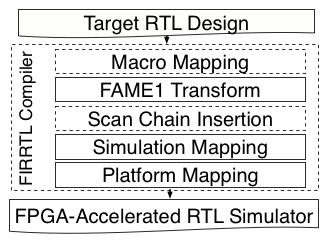
\includegraphics[scale=1.4]{fig4.png}}
		\
		caption{Passos personalizados do compilador para gerar um simulador RTL acelerado por FPGA
		}
		
		\label{Midas Arch}
	\end{figure}
	
	
	Diante disso, a principal função do MIDAS é gerar um simulador de alto desempenho em um alvo a partir de projeto RTL, esse mapeamento pode ser visto na Figura \ref{Mapeamento}. 
	
	\begin{figure}[htbp]
		\centerline{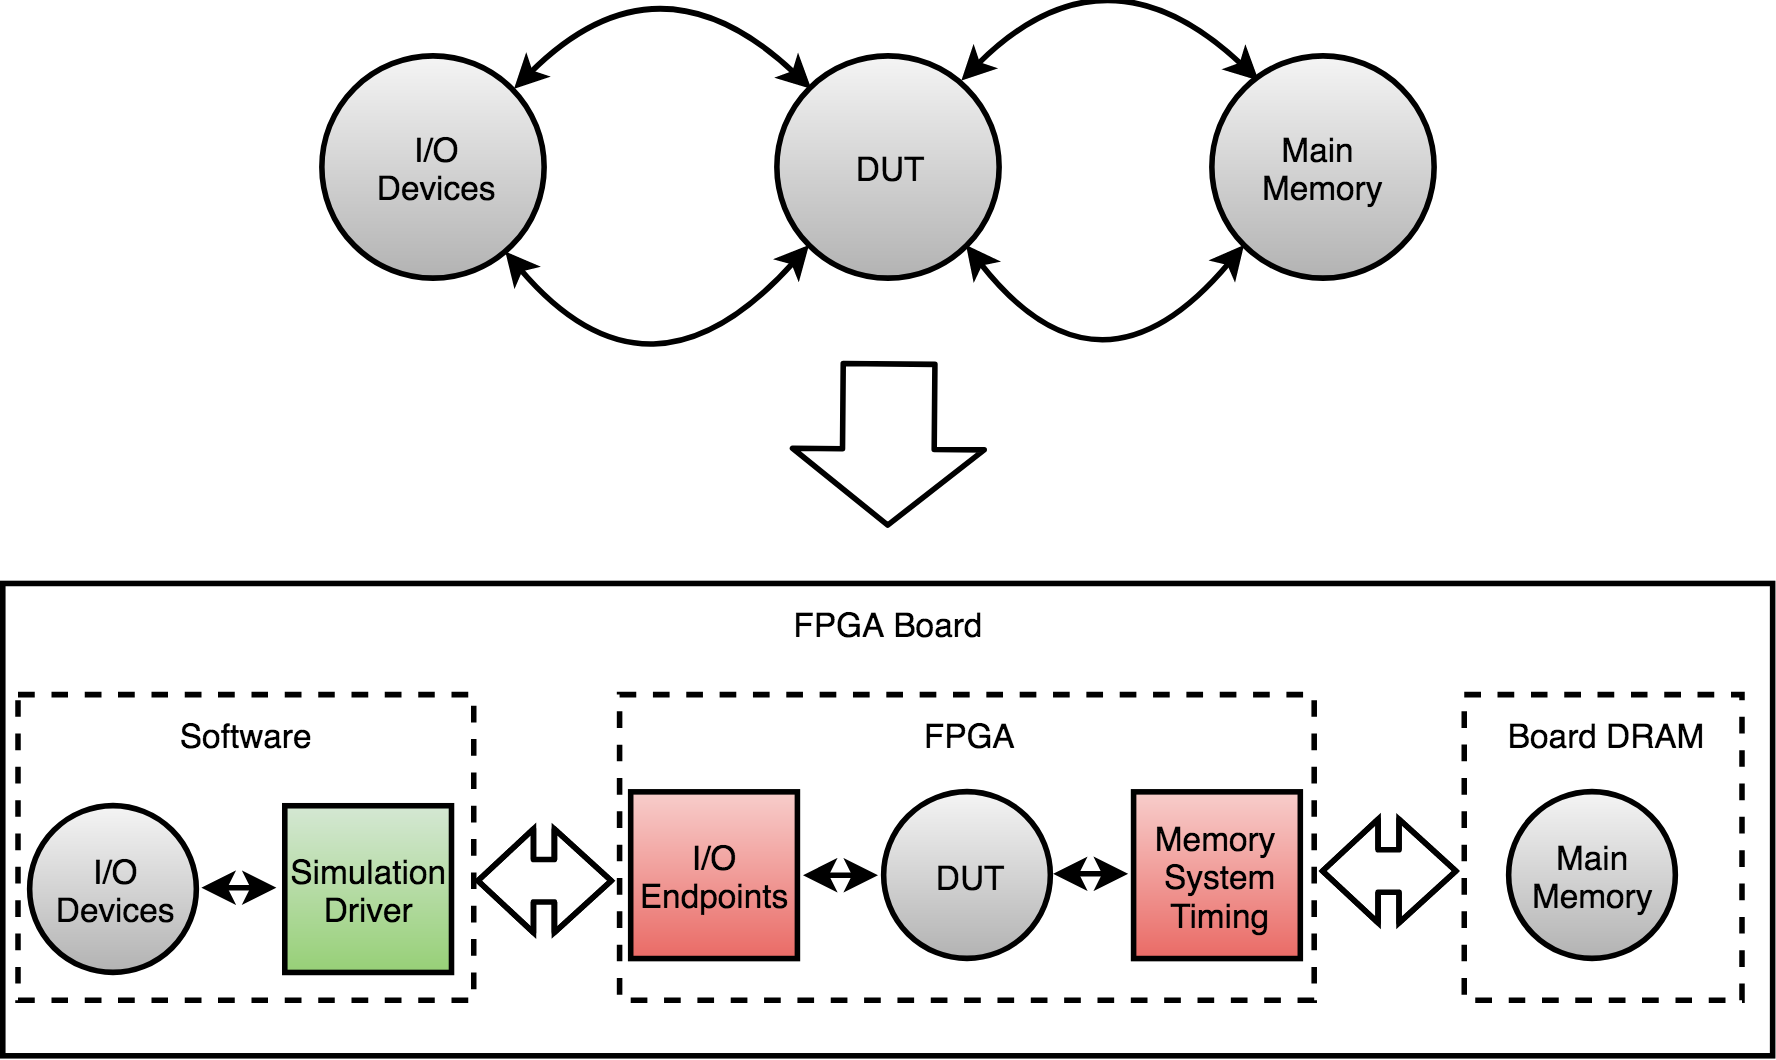
\includegraphics[scale=0.14]{fig2.png}}
		\caption{Mapeamento do projeto alvo para a plataforma de FPGA host -
			Os dispositivo  \textbf{I/O - Devices} são modelados em software e operam ao lado do \textbf{driver de simulação}, pois  as injeções de dados são mais raros.
			Em geral, a comunicação realizada entre a um modelo de software do host e um modelo RTL alvo pos
			sui uma sobrecarga em tempo, por isso existe uma otimização através de  \textbf{I/O- endpoints} , utilizando tokens de tempo que em alto nível  realizam a comunicação com  com o \textbf{DUT} (device under test) utilizando todo o  desempenho de velocidade dos periféricos do FPGA. 
			Dentro do alvo existe um \textbf{modelo de temporização} que tem a função de memória de acesso à \textbf{memória principal}, essa por sua vez está no host.
		}
		
		\label{Mapeamento}
	\end{figure}
	
	
	
	
	
	Uma vez que temos todo o arcabouço para realizar uma simulação rápida em MPSoCs é necessário utilizar ferramentas adequadas para tal, de forma que os requisitos principais dessa simulação sejam atendidos. Com isso é necessário o uso de FPGA com alta velocidade e capacidade de processamento. Esse tipo de dispositivo não é tão acessível, devido ao seu alto custo financeiro. Diante disso, esse trabalho utilizará os recursos de uma FPGA com essas especificações entre outras vantagens, como um serviço no ambiente de nuvem Amazon Web Service(AWS).\\
	A AWS é um plataforma de serviço em nuvem que dispõe de diversos serviços de infra-estrutura, possibilitando usuários ou empresas a utilização desses serviços. A plataforma oferece poder computacional, armazenamento em nuvem distribuição de conteúdo e outros serviços, cada um com sua funcionalidade nas áreas em que são necessários. Dentre esses serviços, existe o EC2F1 que é utilizado para o processamento de dados remoto em FPGAs. O EC2(Amazon Elastic Compute Cloud) é um serviço que fornece acesso aos servidores que possuem os recursos computacionais (essa gerência é realizada sob demanda) , assim o uso do serviço se torna escalável. Um dos tipos de instância EC2 é a EC2 F1, o Amazon EC2 F1 é uma instância de computação com FPGAs que podem ser programadas para criar acelerações de hardware personalizadas para aplicações. Existem outras funcionalidades que essa instância possui, porém este trabalho busca alto desempenho computacional que EC2 F1 disponibiliza. Esse poder de processamento é possível, sobretudo pelas FPGAs que são disponibilizadas na EC2 F1. Essas são Xilinx UltraScale+ VU9P fabricadas em tecnologia de 16 nm, contendo 
	1.182 LUTs, 2.364 flip-flops, 345.9 Mb de memória e 832 de I/O. Vale ressaltar que essa FPGA é caracterizada por possui as mais altas performances entre os dispositivos produtos da Xilinx. Toda a estrutura disponível pela instância, possui uma estratégia de comunicação para realizar a aceleração baseada em FPGA, isso se dá através de conexões via PCIe (PCI Express) com os elementos de CPU (pós-processadores).\\
	Para todo o  processo desenvolvimento de um core AWS, é necessário realizar essas tarefas (figura \ref{aws}):
	\begin{enumerate}
		\item Desenvolver a Lógica Customizada (Custom Logic - CL), que é basicamente o projeto RTL combinado com as ferramentas de desenvolvimento disponíveis na AMI  (Amazon Machine Image) e o HDK (Hardware Development Kit ).
		\begin{enumerate}
			\item FPGA Deveploper
			AMI: Fornece as informações necessárias para executar uma instância, que é um servidor virtual na nuvem. 
			\item Kit de desenvolvimento - HDK: 
			O AWS FPGA HDK é o kit oficial fornecido pela AWS para facilitar o desenvolvimento de RTL (Verilog / VHDL) de uma imagem FPGA da Amazon (AFI).
		\end{enumerate}
		\item Combinar a CL com uma lógica fornecida
		pela AWS chamada de FPGA Shell.
		\begin{enumerate}
			\item FPGA SHELL: É a lógica de plataforma AWS responsável por cuidar dos periféricos externos FPGA, PCIe, DRAM e Interrupções.
		\end{enumerate}
		\item Criar uma Amazon FPGA Image (AFI) a partir da CL construída.
		\begin{enumerate}
			\item AFI: AFI (Amazon FPGA Image) é uma imagem pronta pra ser instanciada na F1, o desenvolvedor pode registrar uma AFI para ser utilizada várias vezes por um uma F1 e/ou pode ser utilizada por várias instâncias F1. 
		\end{enumerate}
		\item Carregar a AFI gerada em uma FPGA conectada à instância F1 ou disponilizar no AWS Marketplace.
		\begin{enumerate}
			\item AWS Marketplace: O AWS Marketplace é uma loja online que ajuda os c
			lientes a descobrir, comprar, migrar e começar a usar imediatamente o software e os serviços de que precisam para criar produtos e gerir suas empresas.  
		\end{enumerate}
	\end{enumerate}
	\begin{figure}[htbp]
		\centerline{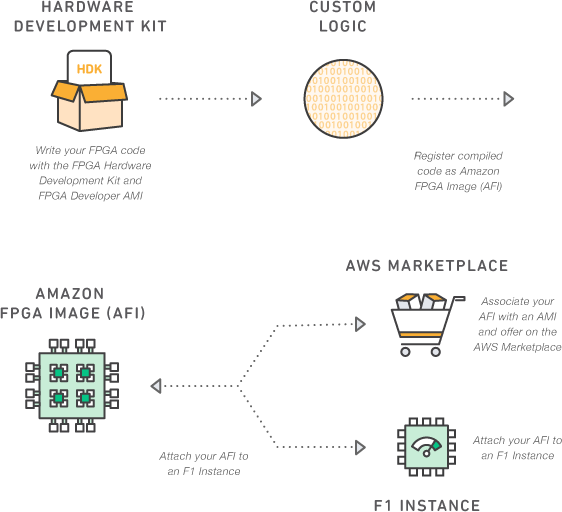
\includegraphics[scale=0.400]{fig3.png}}
		\caption{Processo de desenvolvimento de cores utilizando o serviço EC2 F1 a partir de um projeto RTL}
		\label{aws}
	\end{figure}
	
	\section{Objetivos}
	Tendo em vista o cenário de oportunidades de pesquisa com as ferramentas 
	explicitadas na seção anterior, enumeramos abaixo os objetivos
	gerais e específicos desta pesquisa.\\
	
	\begin{itemize}
		\item Objetivos Gerais\\
		\begin{enumerate}
			\item Propor uma nova metodologia de simulação rápida de MPSoCs, sobretudo do ponto de vista de suas interconexões, tendo em vista que o MIDAS não foi testado em NoCs.
			\item Implementar o modelo proposto em um NoC que utiliza pré-processamento, caracterizando um modelo tolerante a falhas.
			\item Realizar a implementação desse serviço e aceleração do mesmo, utilizando o serviço AWS da Amazon.
			\\
		\end{enumerate}'
		\item  Objetivos Específicos
		\begin{enumerate}
			\item Estudar o modelo da NoC Phoenix com reconfiguração e pré-processamento, além de implementar em uma linguagem a nível RTL suportada pelo MIDAS (Chisel).
			\item Fazer estudo sobre arquitetura MIDAS e outros métodos de aceleração de simulação.
			\item Realizar um estudo do serviço AWS e toda a arquitetura em nuvem necessário para implementação de cores em FPGAs remotos.
			\\
		\end{enumerate}
	\end{itemize}
	
	De acordo com os objetivos pré-estabelecidos, segue abaixo uma tabela que descreve as atividades propostas a serem realizadas nesse projeto, bem como a estimativa de tempo de cada uma.\\
	
	\begin{table}[htbp]
		\caption{TABELA DE ATIVIDADES}
		\begin{center}
			\renewcommand{\arraystretch}{2}% Spread rows out...
			\begin{tabular}{|p{5cm}|c|}
				\hline
				\centering\textbf{Atividade}&\textbf{Estimativa de Tempo} \\
				\hline
				Revisão de literatura sobre NoCs e NoC Phoenix &  Mês 1 e 2  \\
				\hline
				Revisão de literatura sobre da Phoenix resiliente a erros, utilizando pré-processamento,além de sua implementação em VHDL/Verilog&   Mês 3   \\
				\hline
				Revisão de literatura sobre MIDAS e outras aceleradores de simulação& Mês 4  \\
				\hline
				Revisão de literatura sobre o serviço AWS e utilização da EC2 F1& Mês 5  \\
				\hline
				Implementação da Medologia de simulação rápida em MPSoCs& Mês 6 a 12  \\
				\hline
				Testes do Simulador na NoC phoenix, resiliente a erros, utilizando pré-processamento, bem como a implementação no ambiente de nuvem  & Mês 13  \\
				\hline
				Qualificação & Mês 14  \\
				\hline
				Comparação dos resultados obtidos
				com sistemas já existentes & Mês 15 e 16  \\
				\hline
				Escrita para congresso & Mês 17  \\
				\hline
				Escrita da dissertação & Mês 18 a 20  \\
				
				\hline
				
			\end{tabular}
			\label{tab1}
		\end{center}
	\end{table}
	
	\section{Resultados Esperados}
	
	Tendo em vista que as simulações de NoCs com uma maior complexidade (inclusão de técnicas) leva muito tempo para realizar simulações e consequentemente diagnósticos. Esse muitas vezes não é medido de forma mais rigorosa em projetos RTL com simuladores comuns, porém já se sabe que é inviável para uma maior escalabilidades de PEs. Por
	isso esse  pretendemos fazer uma análise do desempenho atual de simulação desse projeto citado, além de propor uma nova solução de simulação eficiente utilizando as ferramentas que foram citadas nesse documento.
	Por fim, para tornar viável  metodologia , se faz necessário a comparação com vários simuladores e com diversos tipos de MPSoCs, tornando a proposta viável em outros cenários de uso.
	
	
	\section*{Referências}
	\renewcommand{\section}[2]{}
	
	\begin{thebibliography}{00}
		\bibitem{b1}  PASRICHA, Sudeep; DUTT, Nikil. On-Chip Communication Architec-
		tures: System on chip interconnect. San Francisco, CA, USA: Morgan Kaufmann Publishers Inc., 2008.
		\bibitem{b2}T. E. Kolding, "A four-step method for de-embedding gigahertz on-wafer CMOS measurements," in IEEE Tra
		nsactions on Electron Devices, vol. 47, no. 4, pp. 734-740, Apr 2000.
		
		\bibitem{b3}R. Marculescu, U. Y. Ogras, L. S. Peh, N. E. Jerger and Y. Hoskote, "Outstanding Research Problems in NoC Design: System, Microarchitecture, and Circuit Perspectives," in IEEE Transactions on Computer-Aided Design of Integrated Circuits and Systems, vol. 28, no. 1, pp. 3-21, Jan. 2009.
		
		\bibitem{b4} Jerraya, A. A.; Wolf, W. "Multiprocessor Systems-on-Chips". Em: Morgan
		Kaufmann Publishers Inc, 2005.
		\bibitem{b5} SILVEIRA, J. et al. Scenario preprocessing approach for the recon-
		figuration of fault-tolerant NoC-based MPSoCs. Microprocessors and
		Microsystems, v. 40, p. 137–153, 2015.
		\bibitem{b6}  STRANO, A. et al. OSR-Lite: Fast and Deadlock-free NoC Reconfi-
		guration Framework. International Conference on Embedded Computer
		Systems (SAMOS), pp. 86-95, 2012.
		\bibitem{b7} C. Marcon, A. Amory, T. Webber, T. Volpato, L. Poehls, Phoenix NoC:
		a distributed fault tolerant architecture, in: International Conference on
		Computer Design (ICCD), 2013.
		\bibitem{b8} Kim, Donggyu, Christopher Celio, David Biancolin, Jonathan Bachrach and Krste Asanovic. “Evaluation of RISC-V RTL with FPGA-Accelerated Simulation.” (2017).
		\bibitem{b9} R. E. Wunderlich, T. F. Wenisch, B. Falsafi and J. C. Hoe, "SMARTS: accelerating microarchitecture simulation via rigorous statistical sampling," 30th Annual International Symposium on Computer Architecture, 2003. Proceedings., 2003, pp. 84-95.
		\bibitem{b10} LI, Patrick S.; IZRAELEVITZ, Adam M.; BACHRACH, Jonathan. Specification for the FIRRTL Language. EECS Department, University of California, Berkeley, Tech. Rep. UCB/EECS-2016-9, 2016.
		\bibitem{b11} Lizhong Chen, Di Zhu, Massoud Pedram, Timothy M. Pinkston, Simulation of NoC
		power-gating: Requirements, optimizations, and the Agate simulator, Journal of Parallel and
		Distributed Computing, Volume 95, 2016, Pages 69-78, ISSN 0743-7315.
		\bibitem{b12} Shin-haeng Kang, Donghoon Yoo, Soonhoi Ha, TQSIM: A fast cycle-approximate
		processor simulator based on QEMU, Journal of Systems Architecture, Volumes 66–67,
		2016, Pages 33-47, ISSN 1383-7621.
		\bibitem{b13} Liana Duenha, Guilherme Madalozzo, Thiago Santiago, Fernando Moraes, Rodolfo
		Azevedo, MPSoCBench: A benchmark for high-level evaluation of multiprocessor systemon-chip
		tools and methodologies, Journal of Parallel and Distributed Computing, Volume
		95, 2016, Pages 138-157, ISSN 0743-7315.
		\bibitem{b14} Koutras, K. Maragos, D. Diamantopoulos, K. Siozios, D. Soudris, On supporting rapid
		prototyping of embedded systems with reconfigurable architectures, Integration, the VLSI
		Journal,Volume 58, 2017, Pages 91-100, ISSN 0167-9260.
		
	\end{thebibliography}
	
	
\end{document}